% !TEX encoding = UTF-8 Unicode
% !TEX TS-program = pdflatex
% !TEX spellcheck = en-US
% !TEX root = ../Report.tex

\chapter{System Linearization}
	Inside this chapter we are going to describe the procedure we adopted in order to get the final Linearized System. We will show our initial approximations and the main step we took into account, starting from the Non-Linear system equations up to the final matrices.
\section{Initial Approximations} \label{approx}
	In order to modify the vehicle behaviour, we decided to act on the steering angles of the rear wheels. Thus, in order to elaborate such control system, we have considered a simplified vehicle model, characterized by the following approximations:
		\begin{itemize}
			\item[1.1] $ \gamma=\dot{\gamma}=0 $: flat plane condition leading to a null vertical acceleration ($ a_{z}=0 $);
			\item[1.2] $\vartheta = \phi = 0$ (Pitch and Roll angles, respectively): the vehicle is leveled with the North-West plane;
			\item[1.3] No Wind and air drag contributions: the aerodynamic force components will be neglected;
		\end{itemize}
\section{Non-Linear System}
	We obtained the two non-linear initial equations starting from the vehicle kinematics equation and both the kinematics and dynamics rotation ones.
\subsection{1st Non-Linear Equation}
	Firstly, we obtained the $\chi$ and $\psi$ math definitions starting from the Vehicle Kinematics Equations (Guidance) combined with both the previous approximations and the under-vehicle side slip angle ($\beta_{u}$) definition. Than, through their geometrical relation, we got the following equation:
		\begin{equation}
			\beta_{u} = \chi - \psi
		\end{equation}
	Derivating the previous equation with respect to time we finally obtained the following statement:
		\begin{equation} \label{Betaudot}
			\dot{\beta}_{u} = \dot\chi - \dot\psi =
			\begin{bmatrix}
			- \sin\beta_{u} & \cos\beta_{u}
			\end{bmatrix}
			\frac{1}{mV_{OB}}
			\begin{bmatrix}
			F_{wx}^{B} \\ F_{wy}^{B}
			\end{bmatrix}
			-\omega_{z}^{B}
		\end{equation}
\subsection{2nd Non-Linear Equation}
	Combining together both the kinematics and dynamics rotation equations and considering $\vartheta = \phi = 0$, we got the following relation describing the rotative dynamics:
	\begin{equation} \label{omegazdot}
		\dot{\omega}_{z}^{B} = \frac{1}{J_{z}} \tau_{z}^{B}
	\end{equation}
	The equations \ref{Betaudot} and \ref{omegazdot} represent, respectively, the 1st and the 2nd equations of the Non-Linear System.
\section{Forces and Moments}
Aiming at describing the vehicle behaviour in a specific situation, we should take into account both the forces and moments acting on it.

Regarding the overall \textit{Forces} typically applied to a generic vehicle, it is possible to split them into three main components: the \textit{gravity} force, the \textit{tire-wheels} forces and the \textit{aerodynamic} ones. In order to simplify our model, as previously said, we have considered some general approximations (see section \ref{approx}, page \pageref{approx}). We will report below the force-related ones:
\begin{itemize}
	\item \textit{Aerodynamic} forces are negligible;
	\item Null vertical acceleration leads to the simple vehicle force weight and its constraint reaction with opposite direction.
\end{itemize}
Given these assumptions, we have obtained a system characterized only by the simple gravitational force of the vehicle and the \textit{tire-wheels} forces (from now on only "\textit{wheels} forces"). Generally, the x-component of the \textit{wheels} forces (\textit{Longitudinal} member) is the sum of both rolling and friction resistances, while the y-one (\textit{Side} member) is only due to friction resistance.
Therefore, for each tire-wheel system of the vehicle, we have to evaluate both the components. \\
There follow the \textit{wheels} forces acting, respectively, along the x,y and z-axis of the i-th tire-wheel system:
\begin{equation} \label{split e roll}
\begin{cases}
F_{wx} = F_{Split} + F_{Rolling} = F_{wz} \mu_{L} + F_{wz} C_{R} \\
F_{wy} = F_{Split} = F_{wz} \mu_{S} \\
F_{wz} = \frac{mg}{4}
\end{cases}
\end{equation}
It is important to emphasize that the relation \ref{split e roll} is true for the i-th wheel. In order to achieve the whole \textit{wheels} force acting over the entire vehicle, we should consider it four times. Within the next steps, we will develop the force equations contained inside the system \ref{split e roll}, in order to better show the most important parameters affecting them.
\newpage
Before going on, let us introduce some key concepts we are going to use. The \textit{Friction Coefficient}, $ \mu $, is defined as follow:
\begin{equation}
\mu = \mu(\lambda_{TOT})
\end{equation}
Moreover, we can specify the \textit{Friction Coefficients} related to both the Longitudinal and the Side slip directions as follow:
\begin{equation}
\begin{cases}
\mu_{L} = \mu(\lambda_{TOT}) \frac{\lambda_{L}}{\lambda_{TOT}}\\
\mu_{S} = \mu(\lambda_{TOT}) \frac{\lambda_{S}}{\lambda_{TOT}}
\end{cases}
\end{equation}
The \textit{Slip} ratio, instead, is responsible to the friction resistance and it is defined by:
\begin{equation}
\lambda_{TOT} = \sqrt{\lambda_{L}^{2} + \lambda_{S}^{2}} \leq 1
\end{equation}
Finally, by merging together all the concepts elaborated so far, we arrived to the following notation:
\begin{equation} \label{Force 1st part}
\begin{bmatrix}
F_{wx} \\
F_{wy}
\end{bmatrix}^{W} =
F_{wz}^{W}
\begin{bmatrix}
\mu_{L} \\
\mu_{S}
\end{bmatrix} =
F_{wz}^{W}
\begin{bmatrix}
\frac{\lambda_{L}}{\lambda_{TOT}} \\
\frac{\lambda_{S}}{\lambda_{TOT}}
\end{bmatrix}
\mu(\lambda_{TOT})
\end{equation}
From the geometric point of view, in terms of reference frames, we can define the \textit{wheels} forces with the following notation:
\begin{equation} \label{Force 2nd part}
\begin{bmatrix}
F_{wx} \\
F_{wy}
\end{bmatrix}^{B} =
R_{BW}
\begin{bmatrix}
F_{wx} \\
F_{wy}
\end{bmatrix}^{W} =
\begin{bmatrix}
\cos\delta_{w} & -\sin\delta_{w} \\
\sin\delta_{w} & \cos\delta_{w}
\end{bmatrix}
\begin{bmatrix}
F_{wx} \\
F_{wy}
\end{bmatrix}^{W}
\end{equation}
Combining together the equations \ref{Force 1st part} and \ref{Force 2nd part}, we obtain the final expression for the \textit{wheels} forces we employed:
\begin{equation} \label{Forces}
\begin{bmatrix}
F_{wx} \\
F_{wy}
\end{bmatrix}^{B} =
\begin{bmatrix}
\cos\delta_{w} & -\sin\delta_{w} \\
\sin\delta_{w} & \cos\delta_{w}
\end{bmatrix}
\frac{F_{wz}^{W} \mu(\lambda_{TOT})}{\lambda_{TOT}}
\begin{bmatrix}
\lambda_{L} \\
\lambda_{S}
\end{bmatrix}
\end{equation}
By processing the above equation \ref{Forces}, we got the two following relations:
\begin{equation} \label{F_{wy}}
\begin{split}
F_{wy}^{B} = 2 [F_{wz}^{W} \mu_{S}\sin\delta_{wr} + (F_{wz}^{W} \mu_{L} + F_{wz}^{W} C_{R}) \cos\delta_{wr}] + \\ + 2 [F_{wz}^{W} \mu_{S}\sin\delta_{wf} + (F_{wz}^{W} \mu_{L} + F_{wz}^{W} C_{R})\cos\delta_{wf}]
\end{split}
\end{equation}
\begin{equation} \label{F_{wx}}
\begin{split}
F_{wx}^{B} = 2 [(F_{wz}^{W} \mu_{L} + F_{wz}^{W} C_{R})\cos\delta_{wr} - F_{wz}^{W} \mu_{S}\sin\delta_{wr}] + \\ + 2 [(F_{wz}^{W} \mu_{L} + F_{wz}^{W} C_{R})\cos\delta_{wf} - F_{wz}^{W} \mu_{S}\sin\delta_{wf}]
\end{split}
\end{equation}

Regarding the overall \textit{Moments} affecting the vehicle behaviour, we simply considered the ones deriving from the forces we took into account. By multiplying them by their own arms we obtained the following general statement:
\begin{equation}
\sum \tau^{B} = \sum r^{B} \sum F_{tire-wheels}^{B}
\end{equation}
The evolution of the previous equation, considering only our parameters of interest, is the following one:
\begin{equation}
\begin{split}
\tau^{B} &= -\omega_{z}(\sum_{i=1}^{2} F_{wz_{i}}^{w} \frac{\mu(\lambda_{TOT_{i}})}{\lambda_{TOT_{i}} V_{max}} (r_{xf}^{2} + r_{yf}^{2}) + \sum_{i=1}^{2} F_{wz_{i}}^{w} \frac{\mu(\lambda_{TOT_{i}})}{\lambda_{TOT_{i}} V_{max}} (r_{xr}^{2} + r_{yr}^{2})) - \\ &- V_{OB}(\sum_{i=1}^{2} F_{wz_{i}}^{w} \frac{\mu(\lambda_{TOT_{i}})}{\lambda_{TOT_{i}} V_{max}} (- r_{yf} \cos \beta_{u} + r_{xf} \sin\beta_{u}) + \\ & + \sum_{i=1}^{2} F_{wz_{i}}^{w} \frac{\mu(\lambda_{TOT_{i}})}{\lambda_{TOT_{i}} V_{max}} (- r_{yr} \cos \beta_{u} + r_{xr} \sin\beta_{u})) + \\ &+ ...
\end{split}
\end{equation}
where "$ ... $" means all those components which do not depend neither on $\beta_{u}$ nor $\omega_{z}$.
\section{Linearization Parameters}
	With the aim of achieve the proper linearized system for our model, we have analyzed the most critical variables affecting the vehicle itself. As a matter o facts, the overall system behaviour is influenced by many parameters, such as vehicle speed ($V_{OB}$), steering angle of both the front ($\delta_{wf}$) and rear ($\delta_{wr}$) wheels , the $\beta_{u}$ angle, and so on. \\
	In order to meet our final purpose, we fixed the following parameters as the reference ones for the linearization process:\\
		\begin{equation*}
			\tilde{x} =
			\begin{bmatrix}
			\beta_{u}^{B} \\\omega_{z}^{B}
			\end{bmatrix} = states \ variables
		\end{equation*}\quad
		\begin{equation*}
			\tilde{u} =
			\begin{bmatrix}
			\delta_{wr}^{B}
			\end{bmatrix} = control \ variable
		\end{equation*}\quad
		\begin{equation*}
			\tilde{d} =
			\begin{bmatrix}
			\delta_{wf}^{B}
			\end{bmatrix} = disturbance \ variables
		\end{equation*}
		\begin{center}
			$ y = output \ variable $
		\end{center}
\section{Linearization Point}
	We chose to linearized our four-wheel steering control system around a straight trajectory of the vehicle. Doing so, we will accept even all those conditions which differ in a way from the previous one. In order to achieve this result, we fixed the following linearization point:
		\begin{equation*}
			\begin{cases}
			\beta_{u} = \dot{\omega_{z}} = 0
			\end{cases}
		\end{equation*}
	In particular, we would like to obtain a stable vehicle, characterized by a constant $\omega_{z}$ based on both the current vehicle speed and front steering angle, imposed by the driver. Moreover, we would obtain the under-vehicle side slip angle as near as possible to the zero value.
\section{Errors Definition}
	Computing the errors means evaluate the dynamic behaviour of the parameters. To make sure we fully clarify what we are going to do, let's define the base elements of each error equation (there follow the ones related to the \textit{states} variable):
		\begin{itemize}
			\item[$\bullet$] $x$ = current state value;
			\item[$\bullet$] $x_{0}$ = equilibrium point;
			\item[$\bullet$] $\tilde{x}$ = small variation of current state.
		\end{itemize}
	Once it has been figured out, there follow the error evaluation for all the considered variables.
		\begin{equation*}
			\begin{cases}
				x = x_{0} + \tilde{x} \\
				u = u_{0} + \tilde{u} \\
				d = d_{0} + \tilde{d} \\
			\end{cases}
		\end{equation*}
	Than, if we simply compute the equivalent time-derivative of each statement, we get:
		\begin{equation*}
			\begin{cases}
				\dot{x} = \dot{x_{0}} + \dot{\tilde{x}} \\
				\dot{u} = \dot{u_{0}} + \dot{\tilde{u}} \\
				\dot{d} = \dot{d_{0}} + \dot{\tilde{d}} \\
			\end{cases}
		\end{equation*}
	Let's compute the \textit{states} relation.\\
	Due to our linearization point, we can rightly say $x_{0} = 0 $, so its time derivative becomes zero as well.
		\begin{equation} \label{matrices structure}
			\begin{split}
				\dot{x}  = \dot{\tilde{x}} &= f(x_{0}+\tilde{x},u_{0}+\tilde{u})\approx \\
				&\approx f(x_{0}+u_{0}) + \frac{\partial f}{\partial x} |_{(x_{0},u_{0})} \tilde{x} + \frac{\partial f}{\partial u} |_{(x_{0},u_{0})} \tilde{u} = \\
				&= 0 + A \tilde{x} + B_{1} \tilde{u}
			\end{split}
		\end{equation}
	Finally, from the equation \ref{matrices structure}, we obtained the origin of each matrix of our system. Inside the next paragraph we are going to elaborate all the partial derivatives within the equation \ref{matrices structure} in order to find each element for all the matrices.

\section{1st Linearized System} \label{1stLinSyst}
	Before starting this section, we will directly show the final structure of our Linear Time-Invariant System we got:
		\begin{equation} \label{LTI}
			\begin{cases}
				\dot{\tilde{x}} = A \tilde{x} + B_{1}\tilde{u} + B_{2}\tilde{d}\\
				y = C\tilde{x}
			\end{cases}
		\end{equation}
	Moreover, inside the next subsections, we are going to describe how we got the 1st version of the above LTI system. It is important to notice that, during the overall design process of our vehicle model, we always kept the system \ref{LTI}'s form as the reference one.
	We will analyze each single matrix, starting from the initial equations followed by our considerations on the parameters the matrices include within them. Furthermore, inside the following section \ref{Final LTI} pag. \pageref{Final LTI}, we will show even the first ever result we obtained considering the 1st LTI system, succeeded by both the issues we faced with and the solutions we adopted to solve them.
\subsection{Matrix $\mathbf{A}$}
	Before showing each element of matrix A, we  need to remind that we started from the two non-linear equations previously described: \ref{Betaudot} and \ref{omegazdot}, respectively. Moreover, since we started with two \textit{state} variables, we have obtained a matrix A $\in M_{2X2}$.\\ There follow the four elements of matrix A:
		\begin{equation} \label{a11}
			a_{11} = \frac{\partial\dot{\beta}_{u}^{B}}{\partial\beta_{u}}\vert_{\beta_{u}=0}  = \frac{1}{mV_{OB}}(F_{wx}^{B} + \frac{\partial F_{wy}^{B}}{\partial\beta_{u}})
		\end{equation}
		\begin{equation} \label{a12}
			a_{12} = \frac{\partial\dot{\beta}_{u}^{B}}{\partial\omega_{z}}\vert_{\dot\omega_{z}=0} = -1 + \frac{1}{mV_{OB}} (F_{wx}^{B} + \frac{\partial F_{wy}^{B}}{\partial\omega_{z}})
		\end{equation}
		\begin{equation} \label{a21}
			a_{21} = \frac{\partial\dot{\omega}_{z}^{B}}{\partial\beta_{u}} = \frac{1}{J_{z}} \frac{\partial\tau_{z}^{B}}{\partial\beta_{u}} \vert_{\beta_{u}=0} = -\frac{1}{J_{z}} V_{0B} (\sum\limits_{i=1}^2 F_{wz_{i}}^{w} \mu(\lambda_{0}) \frac{1}{v_{max}}r_{xf} + \sum\limits_{i=1}^2 F_{wz_{i}}^{w} \mu(\lambda_{0}) \frac{1}{v_{max}}r_{xr})
		\end{equation}
		\begin{equation} \label{a22}
			a_{22} = \frac{\partial\dot{\omega}_{z}^{B}}{\partial\omega_{z}} = \frac{1}{J_{z}} \frac{\partial\tau_{z}^{B}}{\partial\omega_{z}}\vert_{\dot\omega_{z}=0} = -\frac{1}{J_{z}}(\sum\limits_{i=1}^2 F_{wz_{i}}^{w} \mu(\lambda_{0}) \frac{1}{v_{max}} (r_{xf}^{2} + r_{yf}^{2}) + \sum\limits_{i=1}^2 F_{wz_{i}}^{w} \mu(\lambda_{0}) \frac{1}{v_{max}} (r_{xr}^{2} + r_{yr}^{2}))
		\end{equation}
	By combining together the previous components, we got the first  \textit{draft} of matrix $A$.
	\begin{comment}
		\begin{equation}
			A=
			\begin{bmatrix}
				\frac{\partial\dot{\beta}_{u}^{B}}{\partial\beta_{u}^{B}} & \frac{\partial\dot{\beta}_{u}^{B}}{\partial\omega_{z}^{B}} \\
				\frac{\partial\dot{\omega}_{z}^{B}}{\partial\beta_{u}^{B}} & \frac{\partial\dot{\omega}_{z}^{B}}{\partial\omega_{z}^{B}}
			\end{bmatrix} =
			\begin{bmatrix}
				-\frac{1}{mV_{0B}}\frac{\partial F_{y}^{B}}{\partial \beta_{u}}  & -1+\frac{1}{mV_{OB}}\frac{\partial F_{y}^{B}}{\partial \beta_{u}}  \\
				-\frac{1}{J_{z}} V_{0B} (\sum\limits_{i=1}^2 F_{wz_{i}}^{w} \mu(\lambda_{0}) \frac{r_{xf}}{v_{max}} + \sum\limits_{i=1}^2 F_{wz_{i}}^{w} \mu(\lambda_{0}) \frac{r_{xr}}{v_{max}}) &  -\frac{1}{J_{z}}(\sum\limits_{i=1}^2 F_{wz_{i}}^{w} \mu(\lambda_{0}) \frac{(r_{xf}^{2} + r_{yf}^{2})}{v_{max}} + \sum\limits_{i=1}^2 F_{wz_{i}}^{w} \mu(\lambda_{0}) \frac{(r_{xr}^{2} + r_{yr}^{2})}{v_{max}})
			\end{bmatrix}
		\end{equation}
	\end{comment}
\subsection{Matrix $\mathbf{B_{1}}$}
	Following to the theoretical definition of control matrix, by deriving the state's equations with respect to our control variable, $\delta_{wr}^{B}$, we obtained even the first \textit{draft} of matrix $B_{1}$.
		\begin{equation} \label{B1}
			B_{1}=
			\begin{bmatrix}
				\frac{\partial\dot{\beta}_{u}^{B}}{\partial\delta_{wr}^{B}} \\
				\frac{\partial\dot{\omega}_{z}^{B}}{\partial\delta_{wr}^{B}}
			\end{bmatrix} =
			\begin{bmatrix}
				-\frac{1}{mV_{0B}}\{-\sin\beta_{u}\frac{\partial F_{wx}^{B}}{\partial \delta_{wr}} + \cos\beta_{u}\frac{\partial F_{wy}^{B}}{\partial \delta_{wr}}\}  \\
				\frac{1}{J_{z}} \frac{\partial \tau_{z}^{B}}{\partial\delta_{wr}} = \frac{1}{J_{z}} \{ \sum\limits_{i=1}^4 C_{R}F_{wz_{i}}^{w} r_{x_{i}} + \sum\limits_{i=1}^4 F_{wz_{i}}^{w} \mu(\lambda_{0}) \frac{\omega_{i} r}{v_{max}}r_{x_{i}} \}
			\end{bmatrix}
		\end{equation}
	In order to better clarify the equation \ref{B1}, there will follow the forces s partial derivatives components computed without imposing the initial conditions. By doing so, we kept all the parameters of interest inside these equations. In this way, we were able to study the vehicle behaviour simply by changing these parameters inside the Matlab code and analyzing the correspondent consequences. \\ There will follow the x-relative partial derivatives formulas:
		\begin{equation} \label{Fwx su deltaR }
			\begin{split}
				\frac{\partial F_{wx}^{B}}{\partial \delta_{wr}} &= 2 [\frac{\partial F_{wz}^{W}}{\partial \delta_{wr}} (\mu_{L}+C_{R}) \cos\delta_{wr} - F_{wz}^{W} (\mu_{L}+C_{R})\sin\delta_{wr} - \\
				&- \frac{\partial F_{wz}^{W}}{\partial \delta_{wr}} \mu_{S} \sin \delta_{wr} - F_{wz}^{W} \mu_{S}\cos\delta_{wr} - \frac{\partial F_{wz}^{W}}{\partial \delta_{wr}} \mu_{S} \sin \delta_{wf} + \frac{\partial F_{wz}^{W}}{\partial \delta_{wr}} (\mu_{L}+C_{R}) \cos\delta_{wf}]
			\end{split}
		\end{equation}
		\begin{equation} \label{Fwx su deltaF}
			\begin{split}
				\frac{\partial F_{wx}^{B}}{\partial \delta_{wf}} &= 2 [\frac{\partial F_{wz}^{W}}{\partial \delta_{wf}} (\mu_{L}+C_{R}) \cos\delta_{wr} - \frac{\partial F_{wz}^{W}}{\partial \delta_{wf}} \mu_{S} \sin \delta_{wr} + \frac{\partial F_{wz}^{W}}{\partial \delta_{wf}} - (\mu_{L}+C_{R}) \cos\delta_{wf} - \\
				&- F_{wz}^{W} (\mu_{L}+C_{R})\sin\delta_{wf}
				- \frac{\partial F_{wz}^{W}}{\partial \delta_{wf}} \mu_{S} \sin \delta_{wf} - F_{wz}^{W} \mu_{S}\cos\delta_{wf}]
			\end{split}
		\end{equation}
	The next two equations will be the y-relative ones:
		\begin{equation} \label{Fwy su deltaR}
			\begin{split}
				\frac{\partial F_{wy}^{B}}{\partial \delta_{wr}} &= 2 [\frac{\partial F_{wz}^{W}}{\partial \delta_{wr}} \mu_{S} \sin \delta_{wr} + F_{wz}^{W} \mu_{S}\cos\delta_{wf} + \frac{\partial F_{wz}^{W}}{\partial \delta_{wr}} (\mu_{L}+C_{R}) \cos\delta_{wr} + F_{wz}^{W}(\mu_{L}+C_{R}) \sin\delta_{wr}+ \\ &+ \frac{\partial F_{wz}^{W}}{\partial \delta_{wr}} \mu_{S} \sin \delta_{wf} + \frac{\partial F_{wz}^{W}}{\partial \delta_{wr}} (\mu_{L}+C_{R})\cos\delta_{wf}]
			\end{split}
		\end{equation}
		\begin{equation} \label{Fwy su deltaF}
			\begin{split}
				\frac{\partial F_{wy}^{B}}{\partial \delta_{wf}} &= 2 [\frac{\partial F_{wz}^{W}}{\partial \delta_{wf}} \mu_{S} \sin \delta_{wr} + \frac{\partial F_{wz}^{W}}{\partial \delta_{wf}} (\mu_{L}+C_{R}) \cos\delta_{wr} + \frac{\partial F_{wz}^{W}}{\partial \delta_{wf}} \mu_{S} \sin \delta_{wf}+ \\ &+ \frac{\partial F_{wz}^{W}}{\partial \delta_{wf}} (\mu_{L}+C_{R})\cos\delta_{wf} - F_{wz}^{W} (\mu_{L}+C_{R}) \sin\delta_{wf}]
			\end{split}
		\end{equation}
\subsection{Matrix $\mathbf{B_{2}}$}
	Considering that our \textit{disturbance} variable ($\delta_{wf}$) is always a steering angle as the \textit{control} one ($\delta_{wr}$), the processing phase of Matrix $B_{2}$ was exactly the same as the Matrix $B_{1}$ one. \\ The final result, relative to the first \textit{draft}, is reported down here:
		\begin{equation}
			B_{2}=
			\begin{bmatrix}
				\frac{\partial\dot{\beta}_{u}^{B}}{\partial\delta_{f}^{B}} \\
				\frac{\partial\dot{\omega}_{z}^{B}}{\partial\delta_{f}^{B}}
			\end{bmatrix} =
			\begin{bmatrix}
				-\frac{1}{mV_{0B}}\{-\sin\beta_{u}\frac{\partial F_{wx}^{B}}{\partial \delta_{wf}} + \cos\beta_{u}\frac{\partial F_{wy}^{B}}{\partial \delta_{wf}}\} \\
				\frac{1}{J_{z}} \frac{\partial \tau_{z}^{B}}{\partial\delta_{wf}} = \frac{1}{J_{z}} \{ \sum\limits_{i=1}^4 C_{R}F_{wz_{i}}^{w} r_{x_{i}} + \sum\limits_{i=1}^4 F_{wz_{i}}^{w} \mu(\lambda_{0}) \frac{\omega_{i} r}{v_{max}}r_{x_{i}} \}
			\end{bmatrix}
		\end{equation}
	For the elaboration of all the partial derivatives above, refer to subsection \ref{B1}.
\subsection{Matrix C}
	The choice of matrix C was dictated by the math relationship among the x-variable (\textit{states}) and the y-one (\textit{output}) of the system \ref{LTI}, pag. \pageref{LTI}. With the aim of simplifying our system model, we chose the \textit{Identity} matrix to connect these system variables together. \\ In our case, according to both x and y-matrix sizes, we have obtained a matrix C $\in M_{2X2}$.
		\begin{equation}
			C =
			\begin{bmatrix}
				1 & 0 \\
				0 & 1
			\end{bmatrix}
		\end{equation}
	The first \textit{draft} of matrix $C$ and its final version are exactly the same thing.
\section{Final Linearized System} \label{Final LTI}
	We start this section showing our first ever result we obtained by simulating our vehicle model, described inside section \ref{1stLinSyst}, over the pre-defined simulator (it will be better explained inside the chapter \ref{label}).
	The figures \ref{FR traj} and \ref{FR ref} will represent, respectively, the \textit{trajectory comparison} and the \textit{parameters comparison} between closed and open-loop.
\begin{figure}[!b]
	\centering
	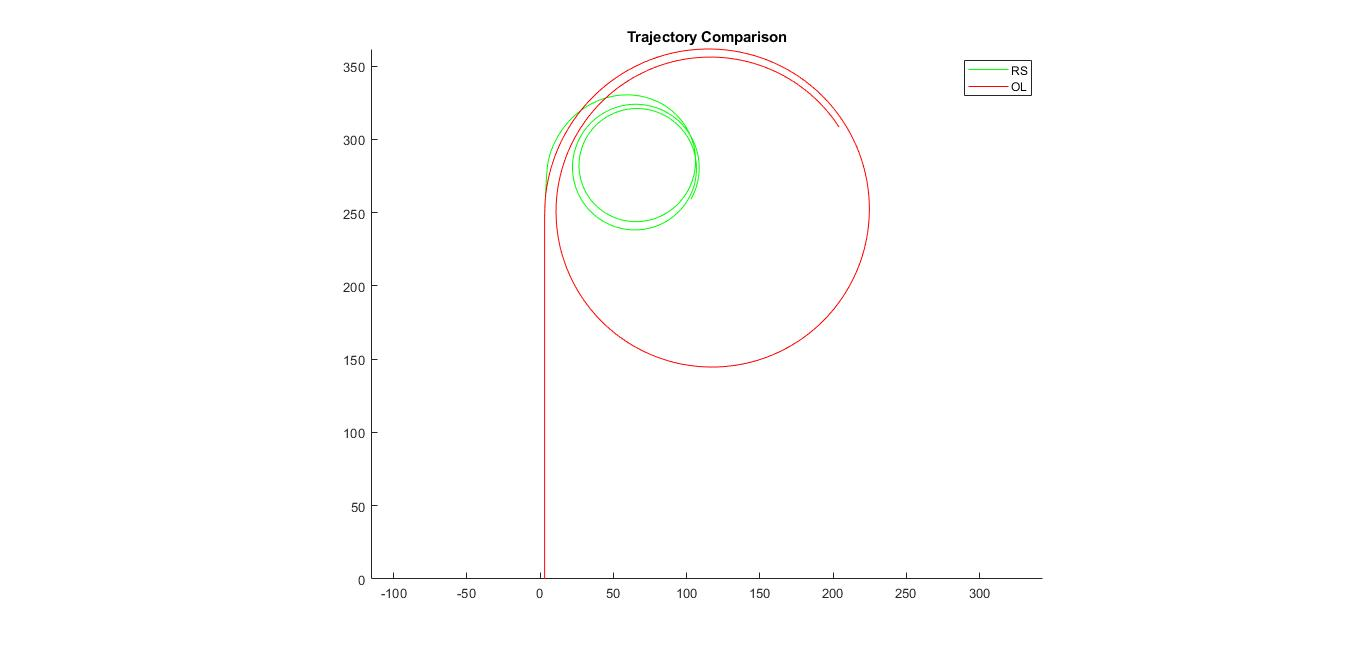
\includegraphics[scale=0.5]{../Images/LinSyst/FakeRes-trj}
	\caption{First ever result - RS vs OL comparison}
	\label{FR traj}
\end{figure}
\begin{figure}
	\centering
	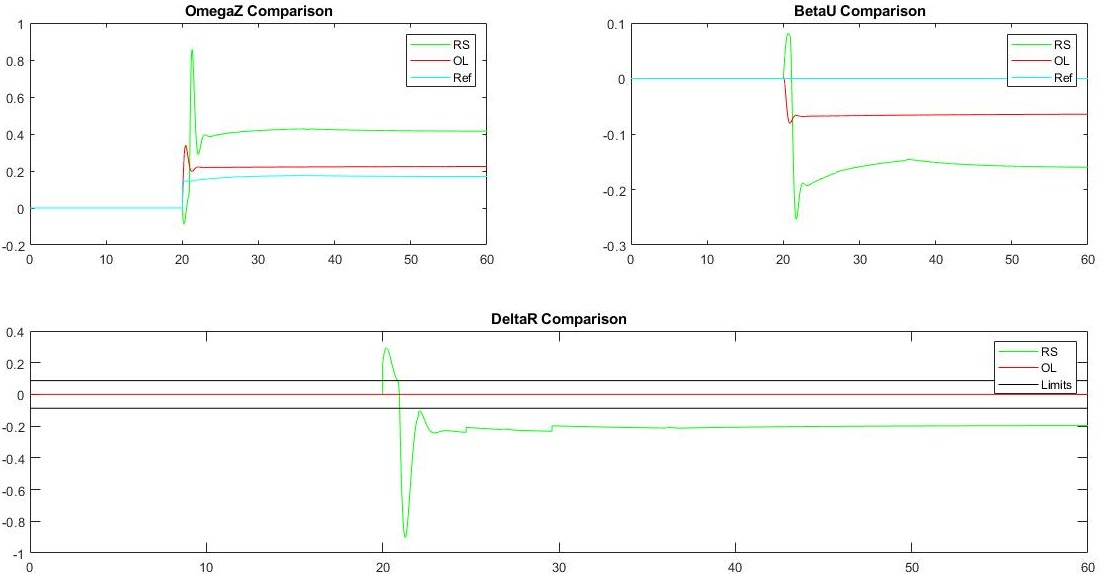
\includegraphics[scale=0.5]{../Images/LinSyst/FakeRes}
	\caption{First ever result - $\omega$, $\beta_{u}$, $\delta_{wr}$ comparison}
	\label{FR ref}
\end{figure}

	Once we achieved that result, we tried to understand which was the root cause leading our control system so far from the reference signal.
	The main problem we noticed was about the differences, in terms of absolute values, between our vehicle model's physical parameters and the pre-defined ones inside the simulator. As a matter of facts, the car included inside the simulator was characterized by different technical parameters, such as weight, center of mass location, moment of inertia and so on. Therefore, our first result was strongly influenced by this technical difference to such an extent that the final vehicle behaviour was not the optimal one.

	To overcome these technical differences in terms of vehicle description, we chose to implement the same physical values of the simulator inside our vehicle model. We did it by inserting a function, inside our Matlab file, calling the needed parameters directly from the simulator database. In this way, we achieved a condition in which, both the simulator and our control system, were working on the same vehicle.

	Moreover, going deeper, we realized that the parameter having the bigger impact on this difference was the cornering stiffness. In particular, we noticed that the vehicle implemented inside the simulator was characterized by fixed values of both front and rear-cornering stiffness, leading to a precise vehicle behaviour. The main consequence of that situation was dictated by a different lateral forces action, due to the side slip angle variation, between our case and the simulator one. For this reason, our first result was not the optimal one. Therefore, as previously said, we implemented the simulator parameters inside our vehicle model to reset such a difference.
	At the beginning, we have not described our LTI system in terms of cornering stiffness. In order to get over this divergence, we have re-written our initial LTI, \ref{Final LTI}, by considering the theoretical definition of cornering stiffness computed in absence of both aerodynamic and rolling friction effects, reported down here (\textit{front} case):
		\begin{equation}
			C_{f} = 2 \mu\lambda_{0}F_{wf}
		\end{equation}
	Moreover, once we checked the cornering stiffness value adopted by the simulator, we notice that it was not multiplied with the friction coefficient. To be perfectly coherent with the theoretical definition, we have implement inside our updated vehicle model, the values displayed inside the fig. \ref{cornering}, where CfRaw and CrRaw are the simulator parameters.
	\begin{figure}[!h]
		\centering
		\lstinputlisting[caption={[Eigenvalues]}, firstline=115, lastline=116, firstnumber=115]{../../../model/LinPlant.m}
		\caption{Lin Plant - Cornering Stiffness definition}
		\label{cornering}
	\end{figure}

	The figure \ref{VehicleScheme} explains how we finally balanced our vehicle, in terms of center of mass location with respect to the wheels axis.
	\begin{figure}
		\centering
		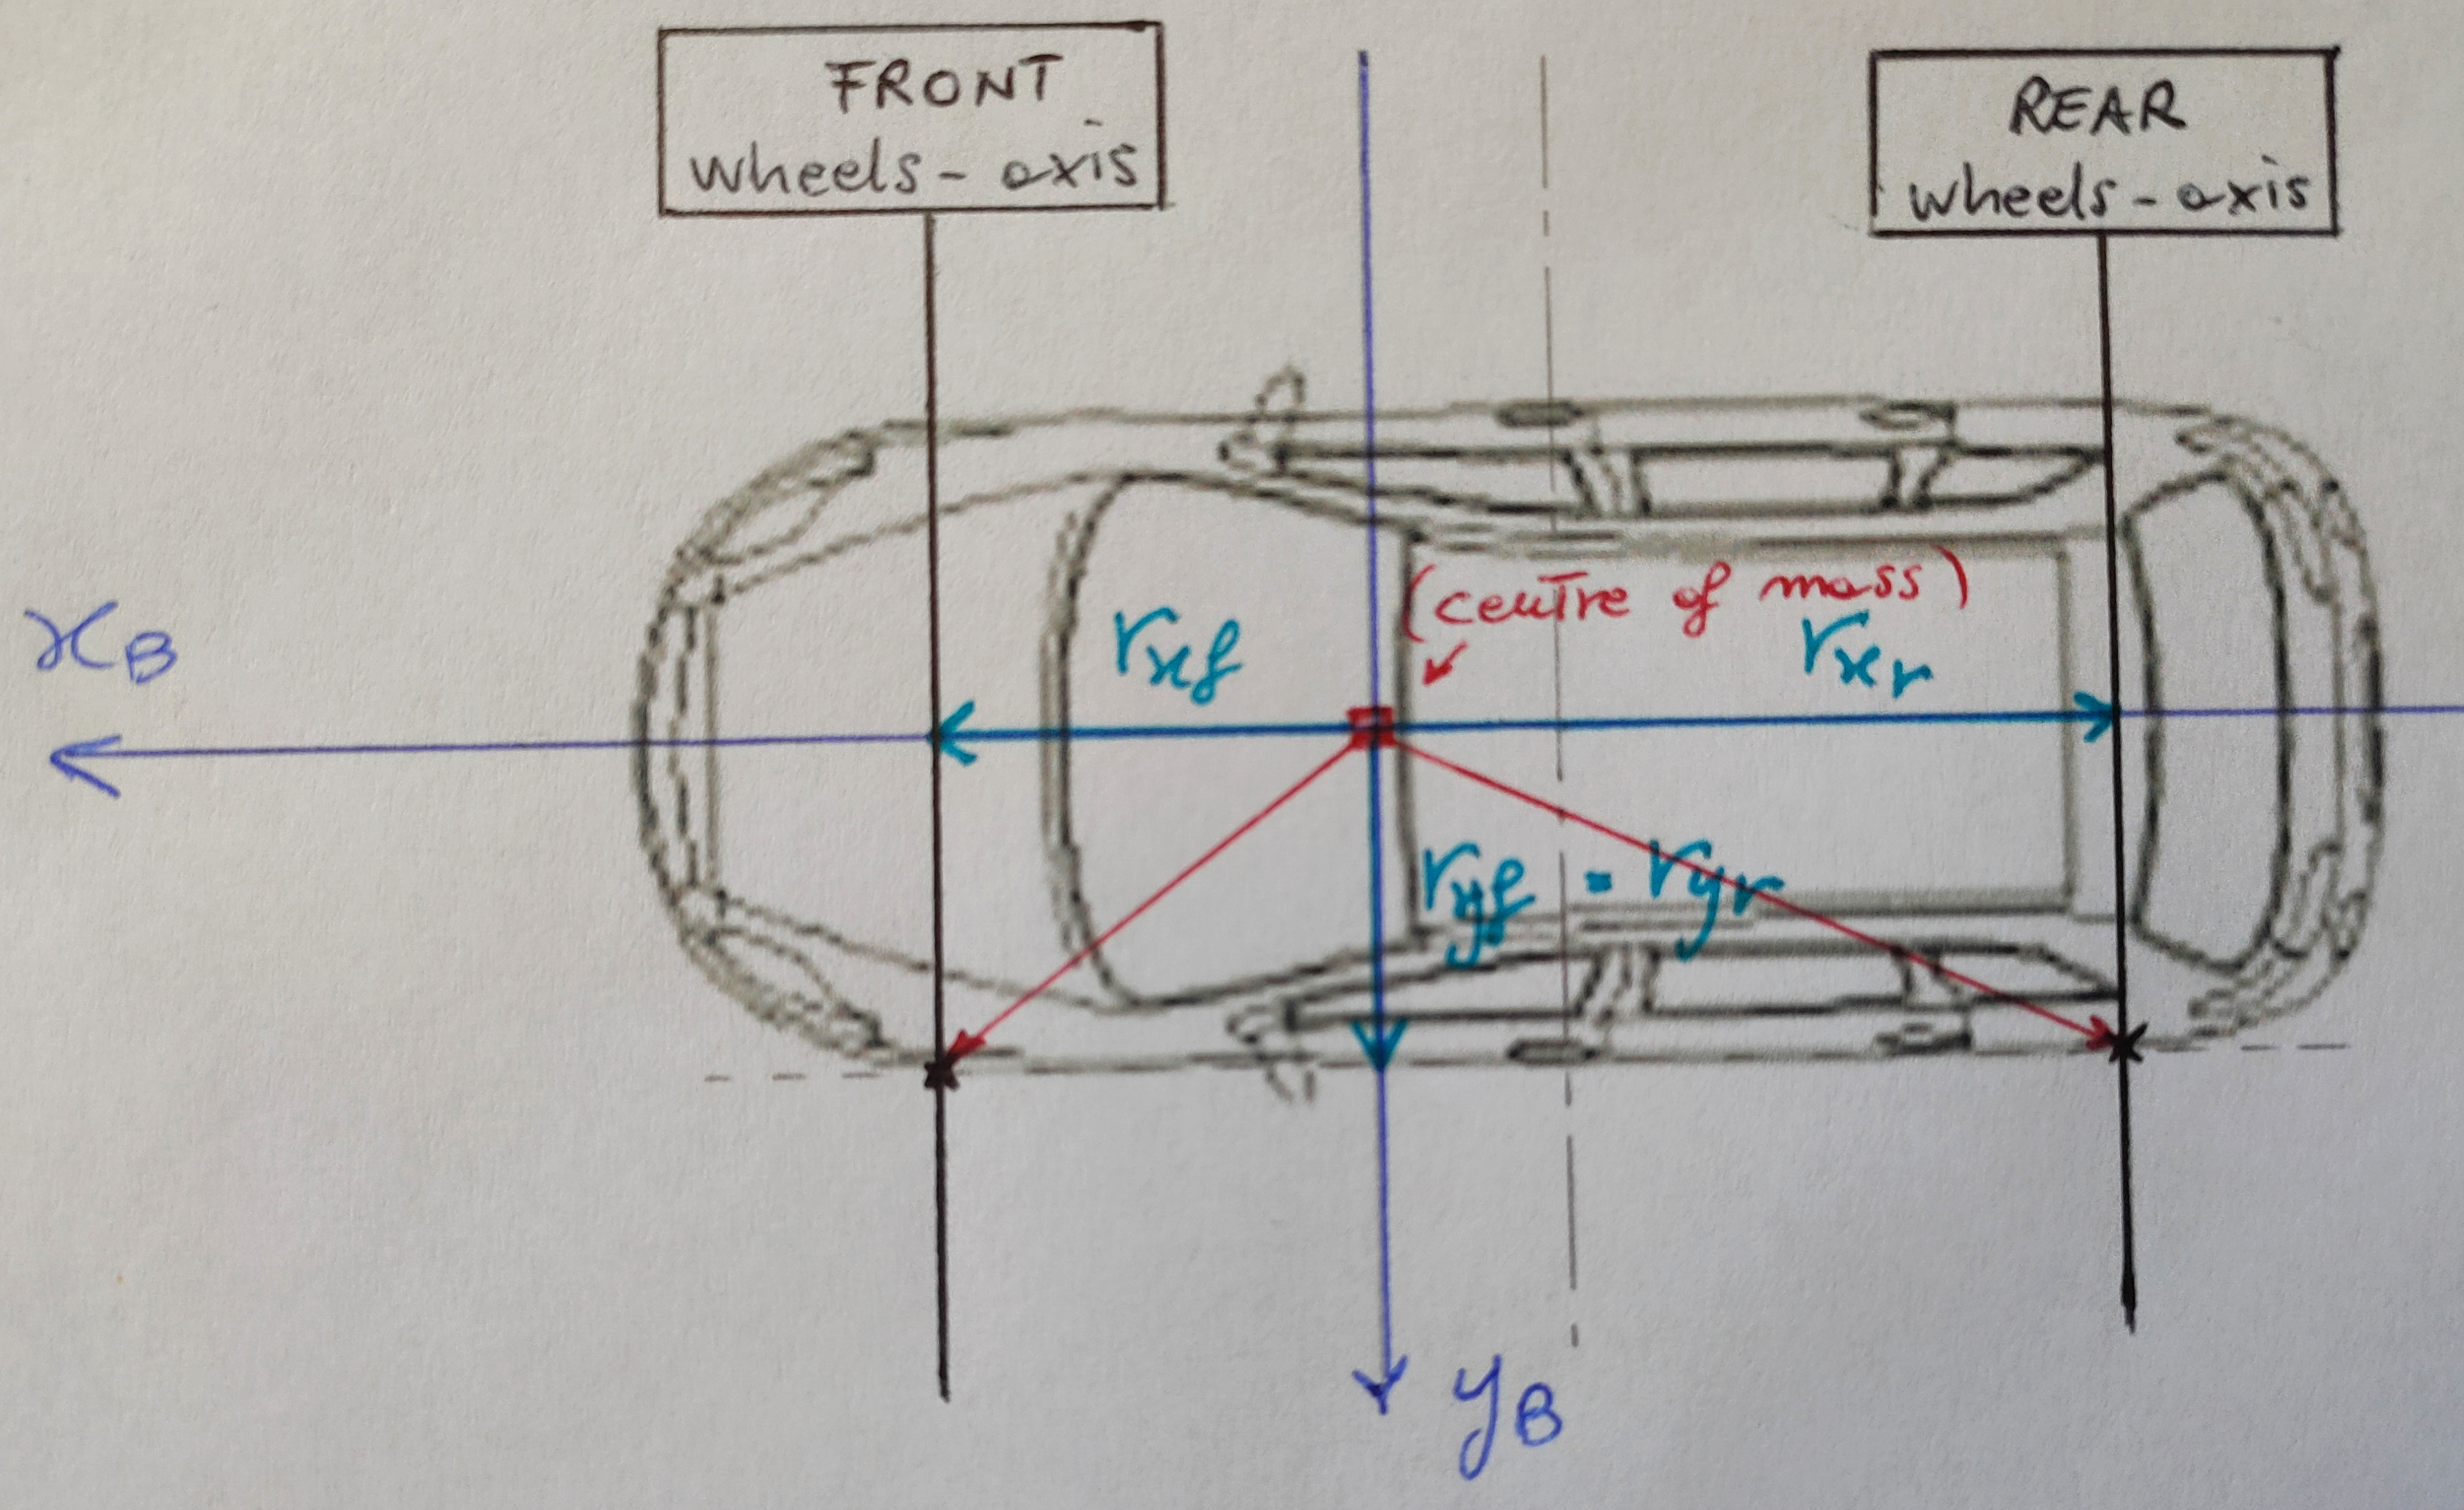
\includegraphics[scale=0.1]{../Images/LinSyst/SchemaAssi}
		\caption{Center of mass - Wheels axis}
		\label{VehicleScheme}
	\end{figure}
\newpage
	Finally, joining together both the last concepts and the \textit{draft} versions of the matrices $A$, $B_{1}$ and $B_{2}$, we got the following final matrices:
\begin{equation}
	A=
	\begin{bmatrix}
		\frac{\partial\dot{\beta}_{u}^{B}}{\partial\beta_{u}^{B}} & \frac{\partial\dot{\beta}_{u}^{B}}{\partial\omega_{z}^{B}} \\
		\frac{\partial\dot{\omega}_{z}^{B}}{\partial\beta_{u}^{B}} & \frac{\partial\dot{\omega}_{z}^{B}}{\partial\omega_{z}^{B}}
	\end{bmatrix} =
	\begin{bmatrix}
		\frac{-(C_{f} + C_{r})}{mV_{0B}} & -1 -\frac{C_{f}r_{xf} + C_{r}r_{xr}}{m V_{0B}^{2}} \\
		-\frac{(C_{f}r_{xf} + C_{r}r_{xr})}{J_{z}} & -\frac{(C_{f}l_{f}^{2} + C_{r}l_{r}^{2})}{J_{z} V_{0B}}
	\end{bmatrix}
\end{equation}
The $B_{1}$ matrix became the following one:
\begin{equation}
B_{1}=
\begin{bmatrix}
\frac{\partial\dot{\beta}_{u}^{B}}{\partial\delta_{r}^{B}} \\
\frac{\partial\dot{\omega}_{z}^{B}}{\partial\delta_{r}^{B}}
\end{bmatrix} =
\begin{bmatrix}
\frac{C_{r}}{m V_{0B}} \\ \frac{C_{r}r_{xr}}{J_{z}}
\end{bmatrix}
\end{equation}
The $B_{2}$ matrix became the following one:
\begin{equation}
B_{2}=
\begin{bmatrix}
\frac{\partial\dot{\beta}_{u}^{B}}{\partial\delta_{f}^{B}} \\
\frac{\partial\dot{\omega}_{z}^{B}}{\partial\delta_{f}^{B}}
\end{bmatrix} =
\begin{bmatrix}
\frac{C_{f}}{m V_{0B}} \\ \frac{C_{f}r_{xf}}{J_{z}}
\end{bmatrix}
\end{equation}
The $C$ matrix, as previously said, was exactly the same one:
\begin{equation}
C =
\begin{bmatrix}
1 & 0 \\
0 & 1
\end{bmatrix}
\end{equation}
